\documentclass[oneside,14pt]{extarticle}
\usepackage[utf8]{inputenc}
\usepackage[english,ukrainian]{babel}
\usepackage{amssymb,amsfonts,amsmath,amsthm,mathtext,textcomp}

\usepackage[includehead, headsep=0pt, footskip=0pt, top=2cm, bottom=2cm, left=2cm, right=1cm]{geometry}
\usepackage{indentfirst}
\usepackage[onehalfspacing]{setspace}
\usepackage[headings]{fancyhdr}
\usepackage{etoolbox}
\usepackage{flafter}
\usepackage{listings}
\usepackage{graphicx}
\usepackage{float}
\usepackage[labelsep=period]{caption}

\usepackage{array}
\fancyhf{}
\renewcommand{\headrulewidth}{0pt}
\pagestyle{fancy}
\fancyfoot[R]{\thepage}
\lstset{breaklines=true,}
\graphicspath{ {./pictures} }

\lstset{
	language=c,
	tabsize=4,
	keepspaces,
	showstringspaces=false,
}
\graphicspath{ {./pictures} }
\setlength{\parindent}{4em}
\setlength\tabcolsep{5px}

\newcommand\subject{Моделювання та аналіз програмного забезпечення}
\newcommand\lecturer{доцент кафедри ПЗ \\ Сердюк П.В.}
\newcommand\teacher{викладач кафедри ПЗ \\ Микуляк А.В.}
\newcommand\mygroup{ПЗ-22}
\newcommand\lab{2}
\newcommand\theme{Linq, List and Dictionary}
\newcommand\purpose{Навчитися працювати з масивами та структурами List, Dictionary.
	Засвоїти технологію LINQ}

\begin{document}
\begin{normalsize}
	\begin{titlepage}
		\thispagestyle{empty}
		\begin{center}
			\textbf{МІНІСТЕРСТВО ОСВІТИ І НАУКИ УКРАЇНИ\\
				НАЦІОНАЛЬНИЙ УНІВЕРСИТЕТ "ЛЬВІВСЬКА ПОЛІТЕХНІКА"}
		\end{center}
		\begin{flushright}
			\textbf{ІКНІ}\\
			Кафедра \textbf{ПЗ}
		\end{flushright}
		\vspace{70pt}
		\begin{center}
			\textbf{ЗВІТ}\\
			\vspace{10pt}
			до лабораторної роботи № \lab\\
			\textbf{на тему}: “\textit{\theme}”\\
			\textbf{з дисципліни}: “\subject”
		\end{center}
		\vspace{50pt}
		\begin{flushright}
			
			\textbf{Лектор}:\\
			\lecturer\\
			\vspace{10pt}
			\textbf{Виконав}:\\
			
			студент групи \mygroup\\
			Коваленко Д.М.\\
			\vspace{10pt}
			\textbf{Прийняв}:\\
			
			\teacher\\
			
			\vspace{28pt}
			«\rule{1cm}{0.15mm}» \rule{1.5cm}{0.15mm} 2023 р.\\
			$\sum$ = \rule{1cm}{0.15mm}……………\\
			
		\end{flushright}
		\vspace{\fill}
		\begin{center}
			\textbf{Львів — 2023}
		\end{center}
	\end{titlepage}
		
	\begin{description}
		\item[Тема.] \theme.
		\item[Мета.] \purpose.
	\end{description}

	\section*{Завдання}
	Для демонстрації роботи розробити Unit-тести для моделі ПЗ відповідно до
	варіанту проекту. Unit-тести повинні створювати списки, словники або інші структури
	об’єктів, та робити із ними різні операції використовуючи LINQ запити.
	
	Як альтернатива Unit-тестам можна використати консольне застосування (для
	максимальної кількості балів таких запитів повинно бути більше).
	\begin{enumerate}
		\item Селекція частини інформації (метод Select)
		\item Вибірка певної інформації (Where)
		\item Операції як з списком List, так і з словником Dictionary
		\item Власні методи розширювання
		\item Використання анонімних класів та ініціалізаторів
		\item Сортування за певним критерієм використовуючи шаблон IComparer
		\item Конвертування списків в масив
		\item Сортування масиву/списку за ім’ям чи за кількістю елементів
	\end{enumerate}

Тести повинні працювати виключно з моделлю об’єктів. Модель об'єктів повинна
включати в себе різні типи даних (чисельні, стрічкові, логічні, множинні і т.д.), для
кожного типу даних повинен бути мінімум 1 тест.

	\section*{Хід виконання}
	
	\begin{figure}[H]
		\centering
		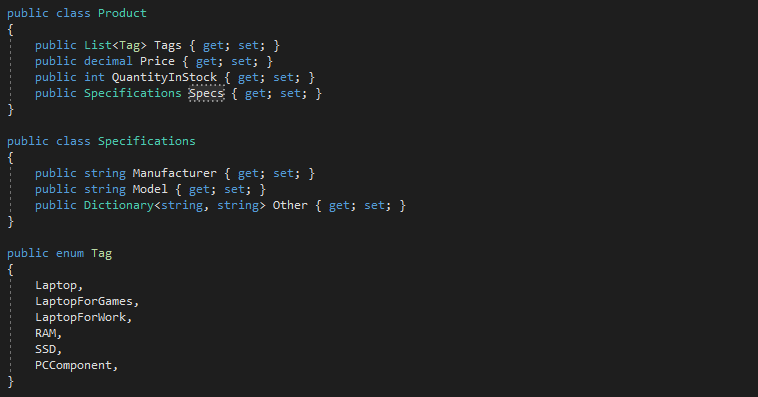
\includegraphics[width=\textwidth]{11}
		\caption{Модель об'єктів}
	\end{figure}

	\begin{figure}[H]
		\centering
		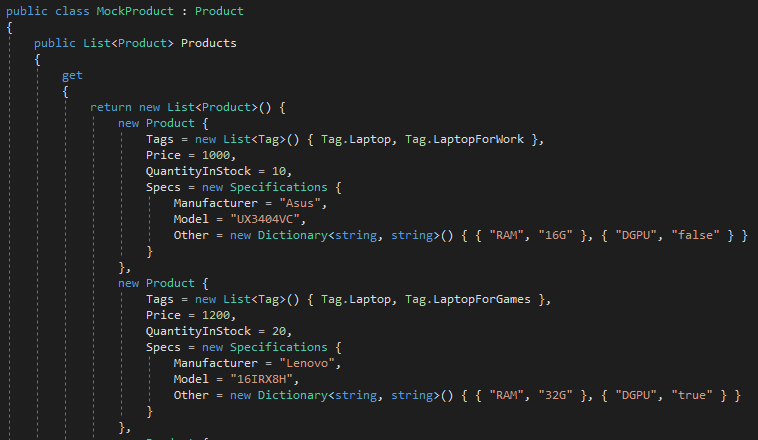
\includegraphics[width=\textwidth]{22}
		\caption{Тестова модель об'єктів}
	\end{figure}
	\begin{figure}[H]
		\centering
		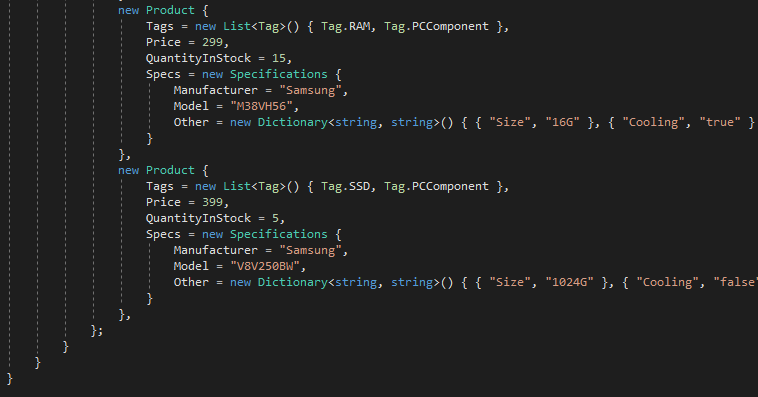
\includegraphics[width=\textwidth]{222}
		\caption{Тестова модель об'єктів}
	\end{figure}

	\begin{figure}[H]
		\centering
		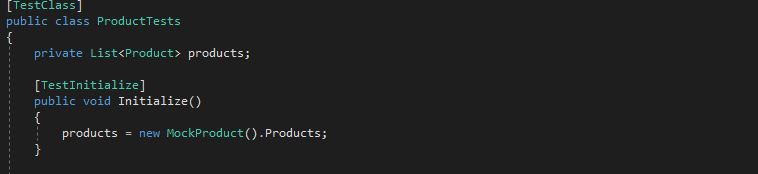
\includegraphics[width=\textwidth]{01}
		\caption{Метод ініціалізації тестів}
	\end{figure}


	\begin{figure}[H]
		\centering
		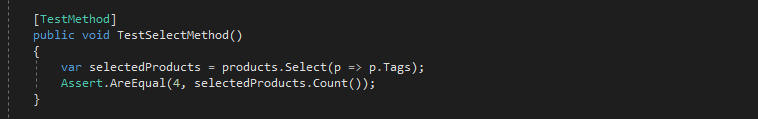
\includegraphics[width=\textwidth]{1}
		\caption{Селекція частини інформації (метод Select)}
	\end{figure}

	\begin{figure}[H]
		\centering
		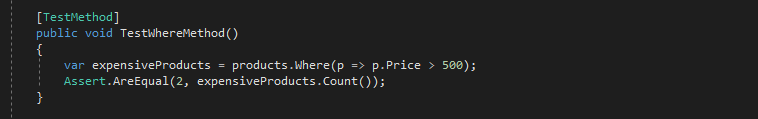
\includegraphics[width=\textwidth]{2}
		\caption{Вибірка певної інформації (Where)}
	\end{figure}
	
	\begin{figure}[H]
		\centering
		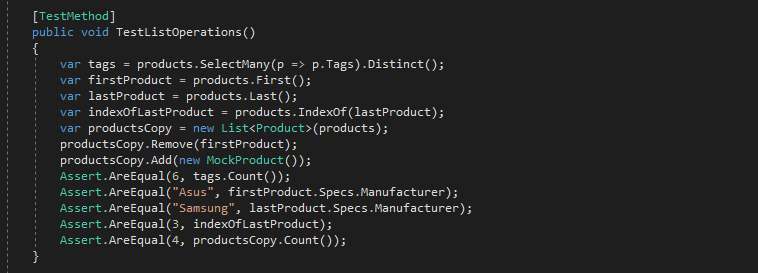
\includegraphics[width=\textwidth]{31}
		\caption{Операції з списком List}
	\end{figure}
	
	\begin{figure}[H]
		\centering
		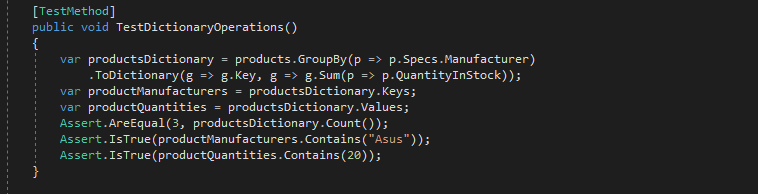
\includegraphics[width=\textwidth]{32}
		\caption{Операції з словником Dictionary}
	\end{figure}
	
	\begin{figure}[H]
		\centering
		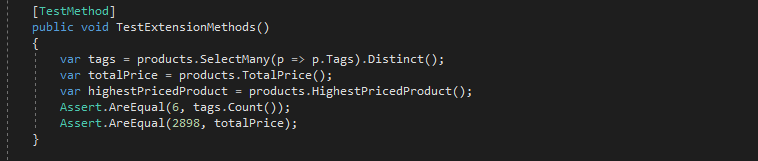
\includegraphics[width=\textwidth]{4}
		\caption{Власні методи розширювання}
	\end{figure}
	
	\begin{figure}[H]
		\centering
		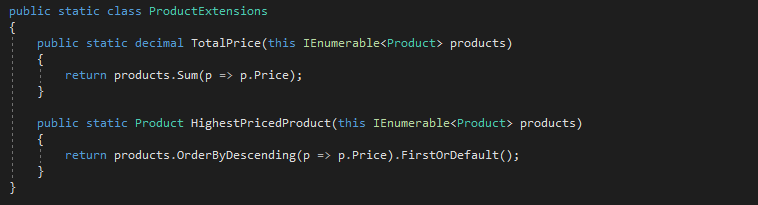
\includegraphics[width=\textwidth]{42}
		\caption{Реалізація власних методів розширення}
	\end{figure}
	
	\begin{figure}[H]
		\centering
		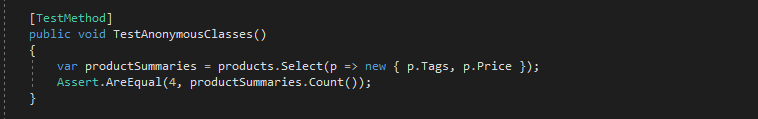
\includegraphics[width=\textwidth]{5}
		\caption{Використання анонімних класів та ініціалізаторів}
	\end{figure}
	
	\begin{figure}[H]
		\centering
		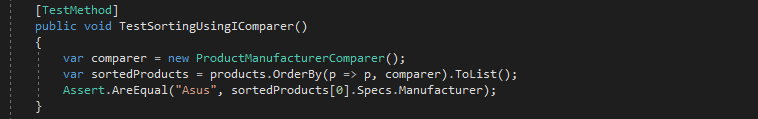
\includegraphics[width=\textwidth]{6}
		\caption{Сортування за певним критерієм використовуючи шаблон IComparer}
	\end{figure}
	
	\begin{figure}[H]
		\centering
		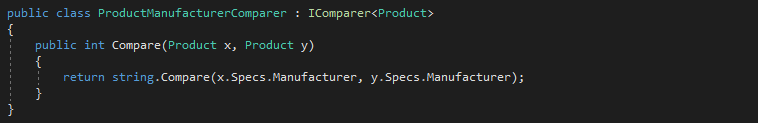
\includegraphics[width=\textwidth]{62}
		\caption{Реалізація інтерфейсу IComparer}
	\end{figure}
	
	\begin{figure}[H]
		\centering
		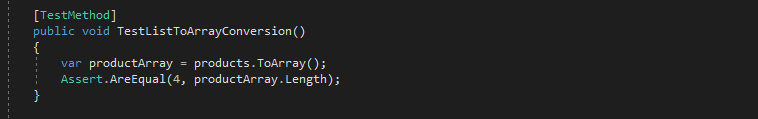
\includegraphics[width=\textwidth]{7}
		\caption{Конвертування списків в масив}
	\end{figure}
	\begin{figure}[H]
		\centering
		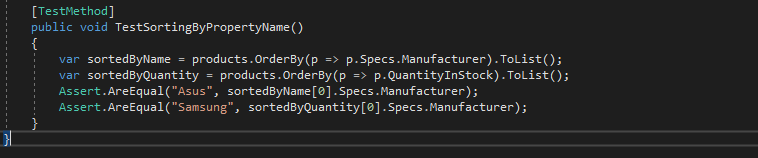
\includegraphics[width=\textwidth]{8}
		\caption{Сортування масиву/списку за ім’ям чи за кількістю елементів}
	\end{figure}
	
	
	\begin{figure}[H]
		\centering
		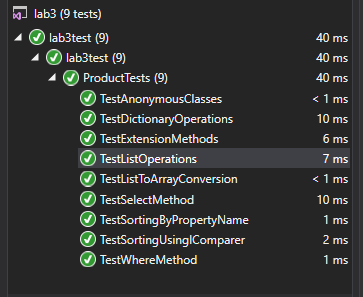
\includegraphics[width=\textwidth]{0}
		\caption{Результат виконання тестів}
	\end{figure}
	
	
	\section*{Висновки}
	   Під час виконання лабораторної роботи я навчився працювати з масивами та структурами List, Dictionary.
	   Засвоїв технологію LINQ.
\end{normalsize}
\end{document}
